\section{Evaluation}
\begin{frame}
     \begin{center}
     	\huge Evaluation 
     \end{center}
\end{frame}

\begin{frame}
\frametitle{Verification Methods}
As that works for partial lists
\begin{itemize}
\item Ranking nDCG
\item Rating nDCG
\item Kendall tau distance 
\item Spearman's footrule distance 
\end{itemize}
\end{frame}

\begin{frame}
\frametitle{Results - Satisfaction Measures}
\small
\begin{adjustwidth*}{-2.1cm}{-2.1cm}
\begin{figure}[h]
\centering
\begin{minipage}{.46\textwidth}\centering
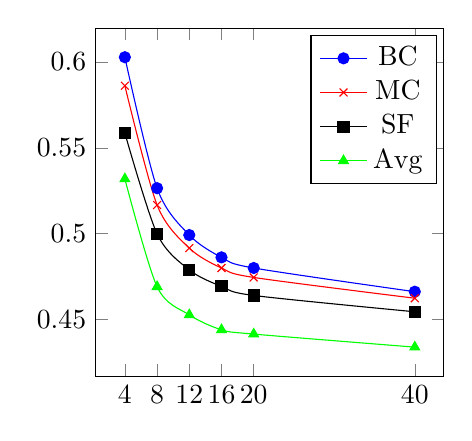
\begin{tikzpicture}
	\begin{axis}[
	height=6cm,
 	width=6cm,
	xtick = {4,8,12,16,20,40}]
	\addplot[smooth,mark=*,blue] plot coordinates {
		(4,0.6028)
		(8,0.5265)
		(12,0.4992)
		(16,0.4862)
		(20,0.48)
		(40,0.4662)
	};
	\addlegendentry{BC}

	\addplot[smooth,color=red,mark=x] plot coordinates {
		(4,0.5862)
		(8,0.5167)
		(12,0.4916)
		(16,0.48)
		(20,0.4745)
		(40,0.4624)
	};
	\addlegendentry{MC}
	
	\addplot[smooth,color=black,mark=square*] plot coordinates {
		(4,0.5586)
		(8,0.4999)
		(12,0.4789)
		(16,0.4693)
		(20,0.464)
		(40,0.4545)
	};
	\addlegendentry{SF}
	
	\addplot[smooth,color=green,mark=triangle*] plot coordinates {
		(4,0.5319)
		(8,0.4691)
		(12,0.4527)
		(16,0.444)
		(20,0.4415)
		(40,0.4339)
	};
	\addlegendentry{Avg}
	
	\end{axis}
	\end{tikzpicture}\captionof{figure}{Ranking nDCG}
\end{minipage}
\begin{minipage}{.58\textwidth}\centering
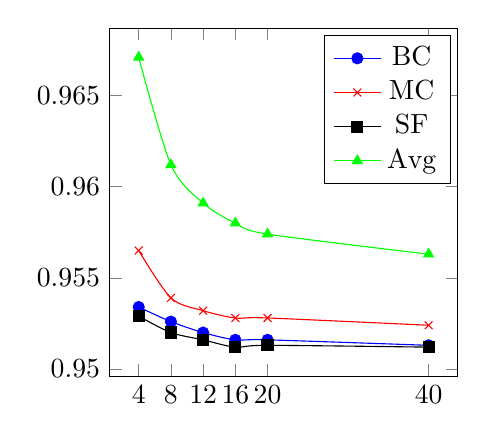
\begin{tikzpicture}
	\begin{axis}[
	height=6cm,
 	width=6cm,
	y tick label style={
        /pgf/number format/.cd,
            precision=3,
        /tikz/.cd
    },
	xtick = {4,8,12,16,20,40}]
	\addplot[smooth,mark=*,blue] plot coordinates {
		(4,0.9534)
		(8,0.9526)
		(12,0.952)
		(16,0.9516)
		(20,0.9516)
		(40,0.9513)
	};
	\addlegendentry{BC}
	
	\addplot[smooth,color=red,mark=x] plot coordinates {
		(4,0.9565)
		(8,0.9539)
		(12,0.9532)
		(16,0.9528)
		(20,0.9528)
		(40,0.9524)
	};
	\addlegendentry{MC}
	
	\addplot[smooth,color=black,mark=square*] plot coordinates {
		(4,0.9529)
		(8,0.952)
		(12,0.9516)
		(16,0.9512)
		(20,0.9513)
		(40,0.9512)
	};
	\addlegendentry{SF}
	
	\addplot[smooth,color=green,mark=triangle*] plot coordinates {
		(4,0.9671)
		(8,0.9612)
		(12,0.9591)
		(16,0.958)
		(20,0.9574)
		(40,0.9563)
	};
	\addlegendentry{Avg}
	
	\end{axis}
	\end{tikzpicture}\captionof{figure}{Rating nDCG}
\end{minipage}
\end{figure}
\end{adjustwidth*}
\normalsize
\end{frame}

\begin{frame}
\frametitle{Results - Distance Measures}
\small
\begin{adjustwidth*}{-2.1cm}{-2.1cm}
\begin{figure}[h]
\centering
\begin{minipage}{.46\textwidth}\centering
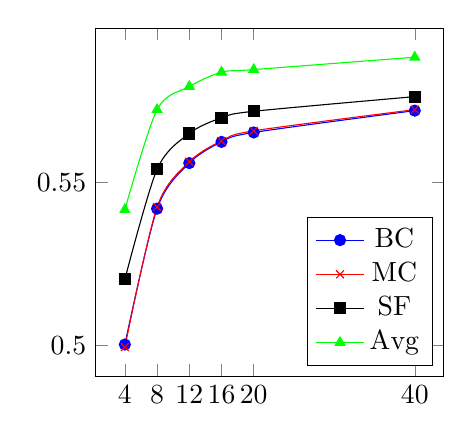
\begin{tikzpicture}
	\begin{axis}[
	height=6cm,
 	width=6cm,
    xtick = {4,8,12,16,20,40},
    legend pos=south east]
    \addplot[smooth,mark=*,blue] plot coordinates {
        (4,0.5002)
        (8,0.5419)
        (12,0.5559)
        (16,0.5624)
        (20,0.5653)
        (40,0.572)
    };
    \addlegendentry{BC}

    \addplot[smooth,color=red,mark=x] plot coordinates {
            (4,0.4994)
            (8,0.5424)
            (12,0.5563)
            (16,0.5627)
            (20,0.5658)
            (40,0.5723)
        };
    \addlegendentry{MC}
    
        \addplot[smooth,color=black,mark=square*] plot coordinates {
            (4,0.5202)
            (8,0.554)
            (12,0.565)
            (16,0.5698)
            (20,0.5718)
            (40,0.5763)
        };
    \addlegendentry{SF}
    
    \addplot[smooth,color=green,mark=triangle*] plot coordinates {
            (4,0.5416)
            (8,0.5723)
            (12,0.5794)
            (16,0.5838)
            (20,0.5846)
            (40,0.5884)
        };
    \addlegendentry{Avg}
    
    \end{axis}
	\end{tikzpicture}\captionof{figure}{Kendall Tau Distance}
\end{minipage}
\begin{minipage}{.58\textwidth}\centering
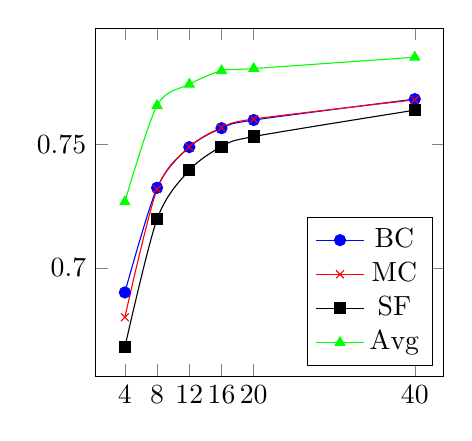
\begin{tikzpicture}
	\begin{axis}[
	height=6cm,
 	width=6cm,
    xtick = {4,8,12,16,20,40},
    legend pos=south east]
    \addplot[smooth,mark=*,blue] plot coordinates {
        (4,0.69)
        (8,0.7325)
        (12,0.749)
        (16,0.7567)
        (20,0.76)
        (40,0.7685)
    };
    \addlegendentry{BC}

    \addplot[smooth,color=red,mark=x] plot coordinates {
            (4,0.6799)
            (8,0.73194)
            (12,0.7491)
            (16,0.7569)
            (20,0.7604)
            (40,0.7682)
        };
    \addlegendentry{MC}
    
        \addplot[smooth,color=black,mark=square*] plot coordinates {
            (4,0.6678)
            (8,0.7198)
            (12,0.7396)
            (16,0.7492)
            (20,0.7533)
            (40,0.764)
        };
    \addlegendentry{SF}
    
    \addplot[smooth,color=green,mark=triangle*] plot coordinates {
            (4,0.7268)
            (8,0.7659)
            (12,0.7745)
            (16,0.78)
            (20,0.7809)
            (40,0.7855)
        };
    \addlegendentry{Avg}
    
    \end{axis}
	\end{tikzpicture}\captionof{figure}{Spearman's Footrule Distance}
\end{minipage}
\end{figure}
\end{adjustwidth*}
\normalsize
\end{frame}

\begin{frame}
\frametitle{Extending Existing Results}
\small
\begin{columns}
\begin{column}{0.5\textwidth}
\begin{figure}
\captionsetup{font=footnotesize}
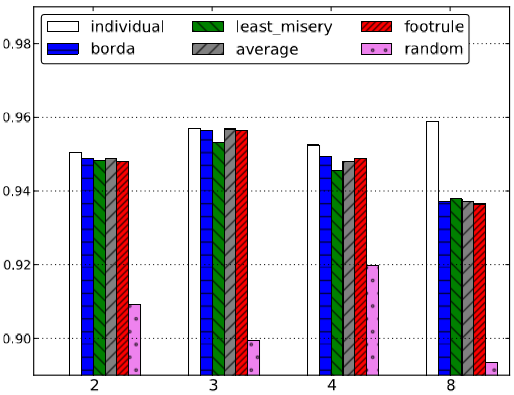
\includegraphics[scale=.45]{graphics/baltruna}
\caption{Rating nDCG from Baltrunas paper\footnote{http://dl.acm.org/citation.cfm?id=1864733}}
\end{figure}
\end{column}
\begin{column}{0.58\textwidth}
\definecolor{bblue}{HTML}{4F81BD}
\definecolor{rred}{HTML}{C0504D}
\definecolor{ggreen}{HTML}{FAAC58}
\definecolor{ppurple}{HTML}{9F4C7C}
\definecolor{ggrey}{HTML}{848484}
\begin{figure}
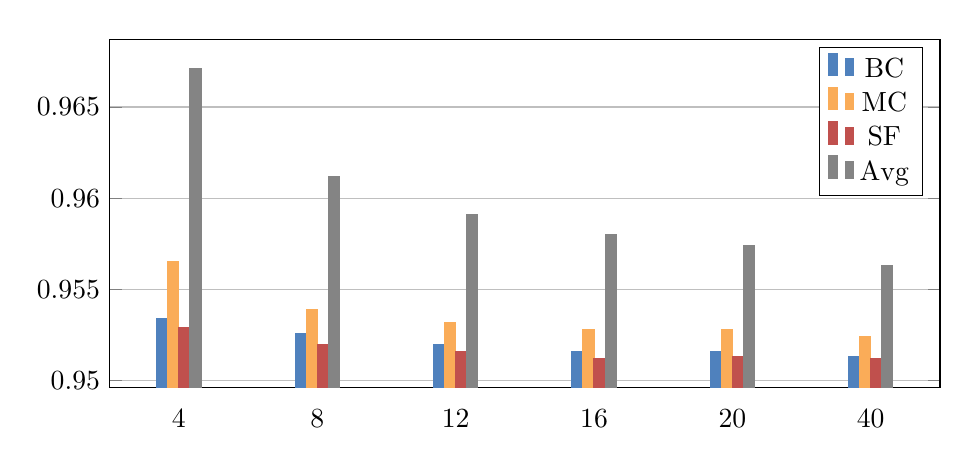
\begin{tikzpicture}
    \begin{axis}[
        width  = 1*\textwidth,
        height = 6cm,
        major x tick style = transparent,
        ybar=0pt,
	y tick label style={
        /pgf/number format/.cd,
            precision=3,
        /tikz/.cd
    },
        bar width=4pt,
        ymajorgrids = true,
        symbolic x coords={4,8,12,16,20,40},
        xtick = data,
        scaled y ticks = false,
    ]
        \addplot[style={bblue,fill=bblue,mark=none}]
            coordinates {
        		(4,0.9534)
        		(8,0.9526)
				(12,0.952)
				(16,0.9516)
				(20,0.9516)
				(40,0.9513)};
				\addlegendentry{BC}
            

        \addplot[style={ggreen,fill=ggreen,mark=none}]
             coordinates {
				(4,0.9565)
				(8,0.9539)
				(12,0.9532)
				(16,0.9528)
				(20,0.9528)
				(40,0.9524)};
            	\addlegendentry{MC}

        \addplot[style={rred,fill=rred,mark=none}]
             coordinates {		(4,0.9529)
				(8,0.952)
				(12,0.9516)
				(16,0.9512)
				(20,0.9513)
				(40,0.9512)
			};
			\addlegendentry{SF}
	
        \addplot[style={ggrey,fill=ggrey,mark=none}]
             coordinates {		
             	(4,0.9671)
				(8,0.9612)
				(12,0.9591)
				(16,0.958)
				(20,0.9574)
				(40,0.9563)
			};
			\addlegendentry{Avg}
    \end{axis}
\end{tikzpicture}
\caption{Rating nDCG}
\end{figure}
\end{column}
\end{columns}
\normalsize
\end{frame}

\begin{frame}
\frametitle{Extending Existing Results}
\small
\begin{columns}
\begin{column}{0.5\textwidth}
\begin{figure}
\captionsetup{font=footnotesize}
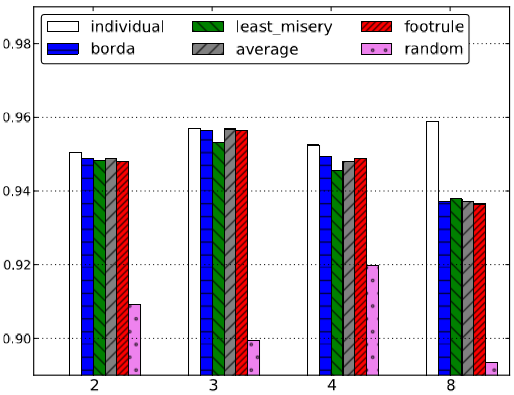
\includegraphics[scale=.45]{graphics/baltruna}
\caption{Rating nDCG from Baltrunas paper\footnote{http://dl.acm.org/citation.cfm?id=1864733}}
\end{figure}
\end{column}
\begin{column}{0.58\textwidth}
\definecolor{bblue}{HTML}{4F81BD}
\definecolor{rred}{HTML}{C0504D}
\definecolor{ggreen}{HTML}{FAAC58}
\definecolor{ppurple}{HTML}{9F4C7C}
\definecolor{ggrey}{HTML}{848484}
\begin{figure}
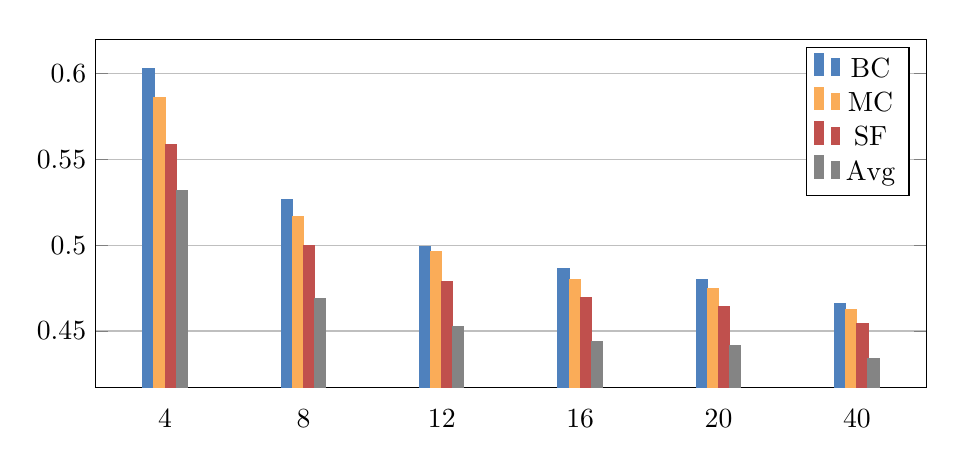
\begin{tikzpicture}
    \begin{axis}[
        width  = 1*\textwidth,
        height = 6cm,
        major x tick style = transparent,
        ybar = 0pt,
	y tick label style={
        /pgf/number format/.cd,
            precision=3,
        /tikz/.cd
    },
        bar width=4pt,
        ymajorgrids = true,
        symbolic x coords={4,8,12,16,20,40},
        xtick = data,
        scaled y ticks = false,
    ]
        \addplot[style={bblue,fill=bblue,mark=none}]
            coordinates {
        		(4,0.6028)
        		(8,0.5265)
				(12,0.4992)
				(16,0.4862)
				(20,0.48)
				(40,0.4662)};
				\addlegendentry{BC}
            

        \addplot[style={ggreen,fill=ggreen,mark=none}]
             coordinates {
				(4,0.5862)
				(8,0.5167)
				(12,0.4961)
				(16,0.4799)
				(20,0.4745)
				(40,0.4624)};
            	\addlegendentry{MC}

        \addplot[style={rred,fill=rred,mark=none}]
             coordinates {		
             	(4,0.5586)
				(8,0.4999)
				(12,0.4789)
				(16,0.4693)
				(20,0.464)
				(40,0.4545)
			};
			\addlegendentry{SF}
	
        \addplot[style={ggrey,fill=ggrey,mark=none}]
             coordinates {		
             	(4,0.5319)
				(8,0.4691)
				(12,0.4527)
				(16,0.444)
				(20,0.4415)
				(40,0.4339)
			};
			\addlegendentry{Avg}
    \end{axis}
\end{tikzpicture}
\caption{Ranking nDCG}
\end{figure}
\end{column}
\end{columns}
\normalsize
\end{frame}